\section{One Wire Driver for the PIC16F54 7 segments
display}\label{one-wire-driver-for-the-pic16f54-7-segments-display}

The Driver control the display over One Wire bus. The driver can set up
the luminosity and shut-down the display. When the driver shutdown the
display, the display can only be startup again from poweron or pushing
the disable/enable-pin down.

The ``PIC16F54 7 segments display'':

\begin{itemize}
\tightlist
\item
  3 x 7 segments common cathode (5611AS)
\item
  1 x PIC16F54 Micro-Controller
\item
  3 x 2n7002 Transistors
\end{itemize}

\subsection{Features}\label{features}

\begin{itemize}
\tightlist
\item
  One wire bus
\item
  Disable/Enable Pin
\item
  Dimming
\item
  Sleep (Energy saving, Then you need two pins)
\item
  3 characters
\end{itemize}

\subsection{Schematic}\label{schematic}

The
\href{documents/images/pic16f54-7-segments-display-schematic.pdf}{schematic}
and the board files

\begin{figure}[htbp]
\centering
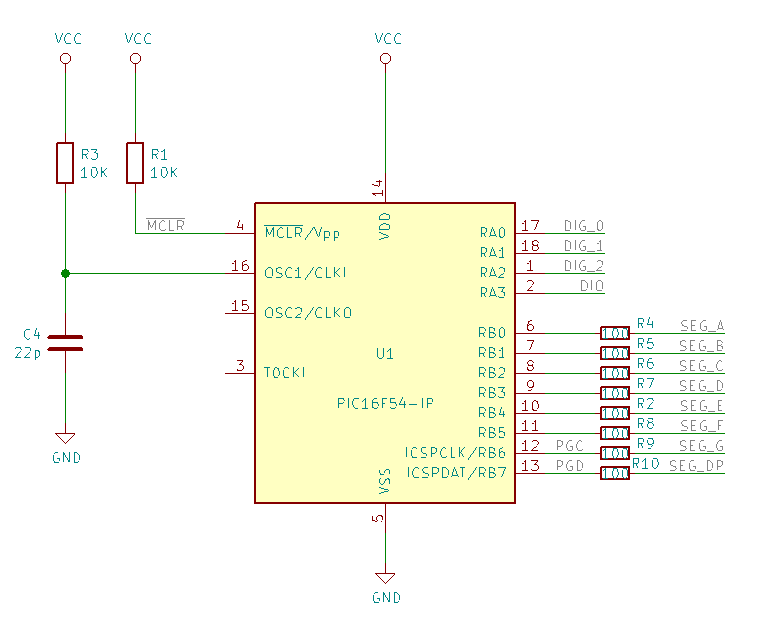
\includegraphics[width=0.80000\textwidth]{documents/images/schematic_mcu.png}
\caption{Schematic MCU\label{schematic_mcu}}
\end{figure}

\begin{figure}[htbp]
\centering
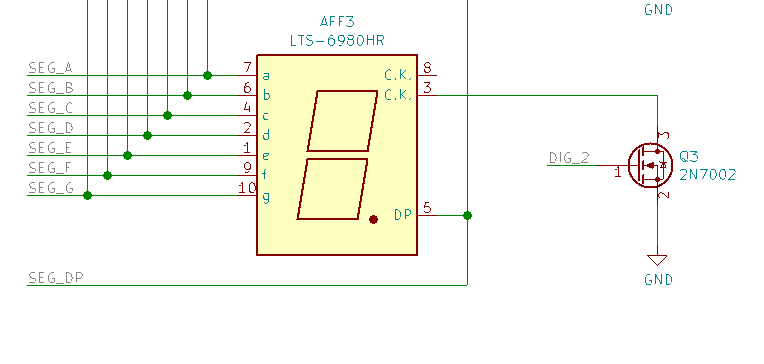
\includegraphics[width=0.80000\textwidth]{documents/images/schematic_seven_segment.png}
\caption{Schematic Seven-Segments\label{schematic_seven_segment}}
\end{figure}

\begin{figure}[htbp]
\centering
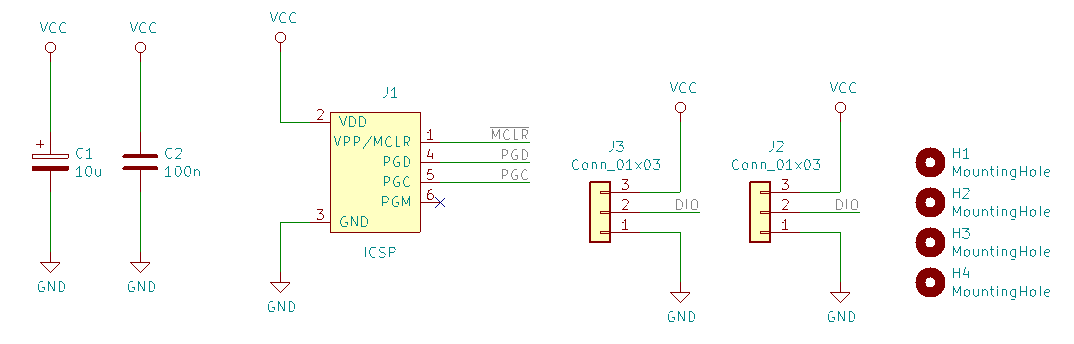
\includegraphics[width=1.00000\textwidth]{documents/images/schematic_seven_prog.png}
\caption{Schematic Programmer and Header\label{schematic_seven_prog}}
\end{figure}

\subsection{One Wire Protocol}\label{one-wire-protocol}

\subsubsection{Bit Timing}\label{bit-timing}

\begin{figure}[htbp]
\centering
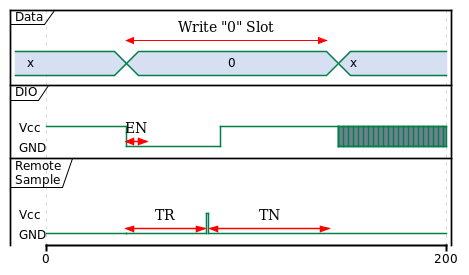
\includegraphics[width=0.80000\textwidth]{documents/images/bit_timing_0.png}
\caption{Master Write ``0'' Slot\label{bit_timing_0}}
\end{figure}

\begin{figure}[htbp]
\centering
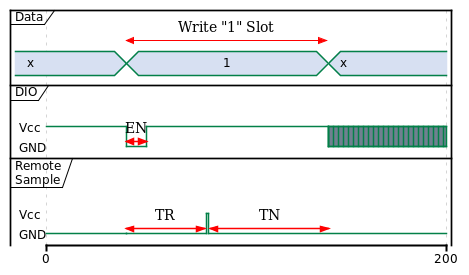
\includegraphics[width=0.80000\textwidth]{documents/images/bit_timing_1.png}
\caption{Master Write ``1'' Slot\label{bit_timing_1}}
\end{figure}

{ The Timings have to be updated! Now the values are just fake values }

\begin{longtable}[c]{@{}cllcrr@{}}
\caption{Bit Timing}\tabularnewline
\toprule
Symbol & Description & Min & Typ & Max & Unit\tabularnewline
\midrule
\endfirsthead
\toprule
Symbol & Description & Min & Typ & Max & Unit\tabularnewline
\midrule
\endhead
EN & Enable & 10 & 10 & 80 & ms\tabularnewline
TR & Time to read & 90 & 100 & 110 & ms\tabularnewline
TN & Time to new bit & 10 & 200 & 220 & ms\tabularnewline
\bottomrule
\end{longtable}

\begin{description}
\tightlist
\item[EN]
Start of new bit
\item[TR]
Time between start of EN and the remote sample the DIO
\item[TN]
Time the remote spend wait for new Data, this should be bigger than the
minimum allowed time for EN
\end{description}

\subsubsection{Command Operation}\label{command-operation}

\begin{figure}[htbp]
\centering
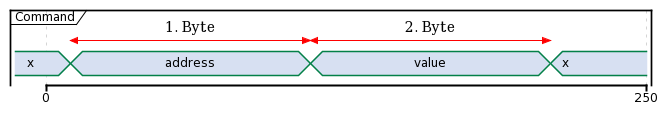
\includegraphics[width=0.80000\textwidth]{documents/images/command.png}
\caption{Command Operation\label{command}}
\end{figure}

\subsubsection{Registers}\label{registers}

\begin{longtable}[c]{@{}lcr@{}}
\toprule
Adresse & Description & Default\tabularnewline
\midrule
\endhead
0x00 & Option & 0x00\tabularnewline
0x01 & Digit 1 & 0x00\tabularnewline
0x02 & Digit 2 & 0x00\tabularnewline
0x03 & Digit 3 & 0x00\tabularnewline
\bottomrule
\end{longtable}

\paragraph{Option Register Bit
Assignement}\label{option-register-bit-assignement}

This register acts as setting register.

\begin{longtable}[c]{@{}ll@{}}
\toprule
One & Two\tabularnewline
\midrule
\endhead
my & table\tabularnewline
is & nice\tabularnewline
\bottomrule
\end{longtable}

\begin{longtable}[c]{@{}lcccccccc@{}}
\caption{Option Register}\tabularnewline
\toprule
Option & 7 & 6 & 5 & 4 & 3 & 2 & 1 & 0\tabularnewline
\midrule
\endfirsthead
\toprule
Option & 7 & 6 & 5 & 4 & 3 & 2 & 1 & 0\tabularnewline
\midrule
\endhead
& SLEEP & EN & DIM5 & DIM4 & DIM3 & DIM2 & DIM1 & DIM0\tabularnewline
Default & 0 & 0 & 0 & 0 & 0 & 0 & 0 & 0\tabularnewline
\bottomrule
\end{longtable}

\begin{description}
\tightlist
\item[DIM\textless{}5-0\textgreater{}]
Dimmer, `0b000000' is full power and `0b111111' is dark.
\item[EN]
Writing `1' to this position will power off the segments. All segments
are off, but the controller is still running.
\item[SLEEP]
The controller go in sleep. Can only be restart push the MCLR pin down.
All registers will be reset to theirs default value.
\end{description}

\paragraph{Digit x Register Bit
Assignement}\label{digit-x-register-bit-assignement}

Registers describing the segments that should light on. Writing `1' to a
position will light on this segments.

\begin{longtable}[c]{@{}cccccccc@{}}
\toprule
Bit 7 & Bit 6 & Bit 5 & Bit 4 & Bit 3 & Bit 2 & Bit 1 & Bit
0\tabularnewline
\midrule
\endhead
DP & G & F & E & D & C & B & A\tabularnewline
\bottomrule
\end{longtable}

\begin{figure}[htbp]
\centering
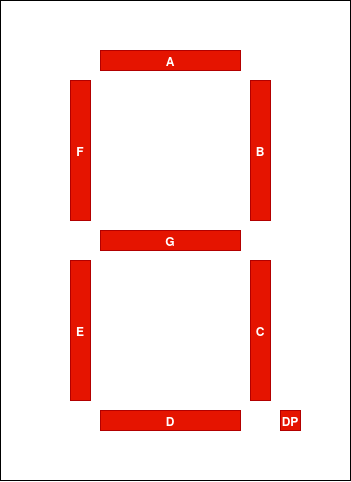
\includegraphics[width=0.50000\textwidth]{documents/images/seven_segments.png}
\caption{Seven Segments\label{command}}
\end{figure}

\subsection{To-Do}\label{to-do}

\begin{itemize}
\tightlist
\item
  {[}x{]} Implement power off the segments (Bit 6 of option register)
\item
  {[} {]} Update Bit-Timing with the right value
\end{itemize}
